%\documentclass[]{article}
%\usepackage{graphicx}
%\usepackage{subfig}
%\usepackage{amsmath}
%\usepackage{amsfonts}
%\usepackage[margin=1in]{geometry}

%\begin{document}


First, it's worth understanding how basic characteristics of our dataset respond to dimensionality reduction.  In figure \ref{fig:PCA_RED} we estimate a 500-dimensional PCA projection (computing more principle components than 500 was intractable on our high-dimensional dataset). Next, we truncate this to a smaller-dimensional projection, and see how aspects of the data scale with projection size. In  \ref{fig:PCA_RED}(a) we compute the total covariance of the first 500 principle components, and then show what fraction of this total covariance is captured as we increase the dimensionality of the projection. We find that the curve grows quite slowly. In order to capture 50\% of the total covariance, we need to use about 150 principle components. In  \ref{fig:PCA_RED}(b) we measure the sparsity (percentage of zero entries) of the projected design matrix. The raw matrix unprojected matrix is 99.6\% sparse. We find that the sparsity increases quite quickly with PCA projection dimension. Therefore, if we want to capture a reasonable amount of the total covariance, we must deal with very sparse data. 

\begin{figure}[!ht]
\centering
\subfloat[Cumulative Cov. vs. dim PCA]{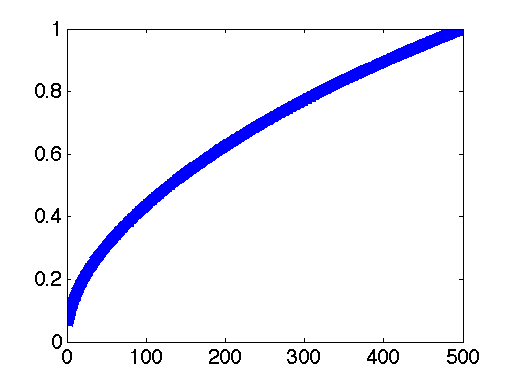
\includegraphics[width=.33\textwidth]{../images/pca_cumsum.png}}
\subfloat[Zoom-in of Cum. Cov. vs. dim PCA]{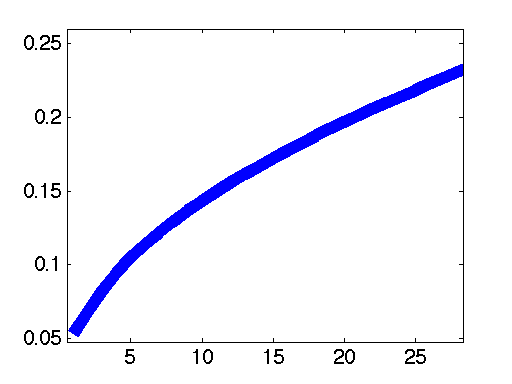
\includegraphics[width=.33\textwidth]{../images/pca_cumsum_zoom.png}}
\subfloat[Data Sparsity vs. dim PCA]{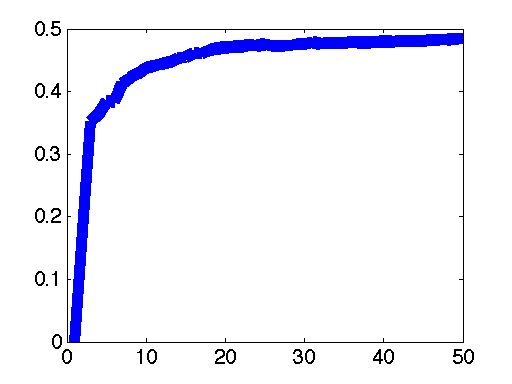
\includegraphics[width=.33\textwidth]{../images/PCAsparsityDensity.png}}
\caption{Characteristics of PCA-reduced data}
\label{fig:PCA_RED}
\end{figure}

Due to this tradeoff between data sparsity and representation of the raw data's variation, it is unclear what the optimal PCA projection dimension is. In figure \ref{fig:pca_acc_vs_proj_dim}, we vary the projection dimension and plot the accuracy of two different classifiers. 

In \ref{fig:pca_acc_vs_proj_dim}(a), we use Naive Bayes, with `add one' smoothing, where a certain number of rows of all ones are added to the design matrix. We choose the number of pseudocounts for these added rows by optimizing classification performance on a development set. Pseudocount optimization is done separately for each PCA dimension, in order to count for the changing sparsity of the data. We find that accuracy peaks when using a 7-dimensional projection. Considering figure  \ref{fig:PCA_RED}, this is unsurprising, because it is around this dimension where the sparsity of the data increases considerably. 

In contrast, in \ref{fig:pca_acc_vs_proj_dim}(b), we use an linear-kernel SVM, which is less sensitive to data sparsity. In contrast with naive Bayes, accuracy stays high when increasing PCA dimension. SVM model complexity scales with the number of training points, not the dimensionality of the input space. Therefore, there is less of a concern when increasing projection dimensionality, and performance increases because in a higher-dimensional projected space, pairwise distances between points are captured with higher fidelity. 

\begin{figure}[!ht]
\centering
\subfloat[Naive Bayes acc. vs. PCA dim]{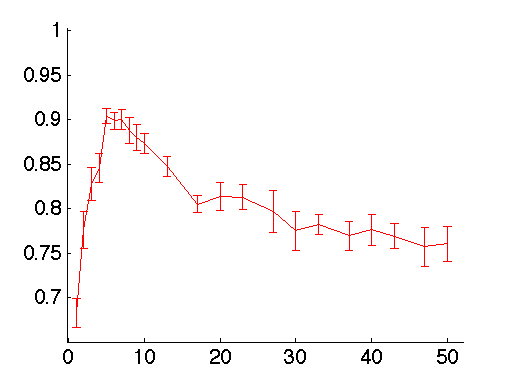
\includegraphics[width=.5\textwidth]{../images/nb_acc_vs_dim_pca_sr.png}}
\subfloat[SVM acc. vs. PCA dim]{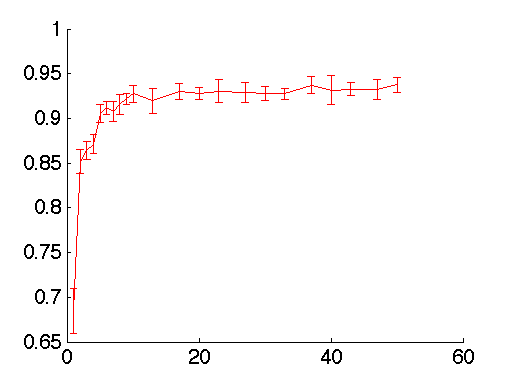
\includegraphics[width=.5\textwidth]{../images/svm_acc_vs_dim_pca_sr.png}}
\caption{Accuracy vs. dim. PCA Projection}
\label{fig:pca_acc_vs_proj_dim}
\end{figure}

TODO add a note that when we do random projections and increase dimensionality we keep the p-1 previous projection dimensions fixed. 

\begin{center}
\begin{figure}[!ht]
\centering
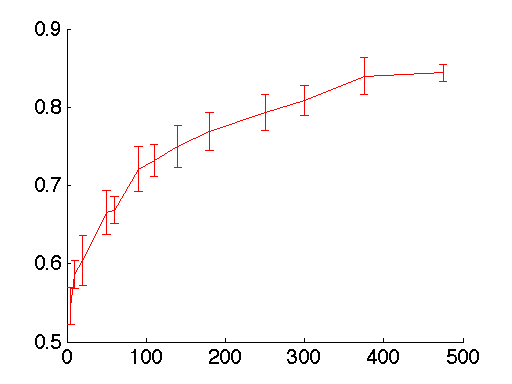
\includegraphics[width=.5\textwidth]{../images/accuracy_vs_dim_randproj.png}
\caption{Naive Bayes Acc. vs. num dim Rand. Projection}
\label{fig:nb_rand_proj}
\end{figure}
\end{center}


	Next, in figure \ref{fig:distance}(a), we explore how the curse of dimensionality affects k-nearest neighbors (KNN) and performing KNN on projected data. We compare 3 scenarios: unprojected 17,000 dimensional data (red), PCA-reduced data (blue), randomly projected data (green). We vary the dimensionality of the projection for the PCA and random projection datasets. We find that  PCA improves KNN over using no projection, even for PCA dimensions as high as 80. 

	The fact that PCA helps may be a consequence of the curse of dimensionality. In higher dimensional spaces, there is less variation among pairwise distances, so classifiers based on pairwise distances may perform worse. To support this claim, in figure ~\ref{fig:distance}(b) we conduct a similar experiment varying PCA dimension, but contrast an the classification accuracy of an SVM with a linear kernel and one with a radial basis kernel. As expected, we find that classification performance with the radial basis kernel decreases with PCA dimension. 

\begin{figure}[!ht]
\centering
\subfloat[Accuracy vs Dim. proj  with KNN]{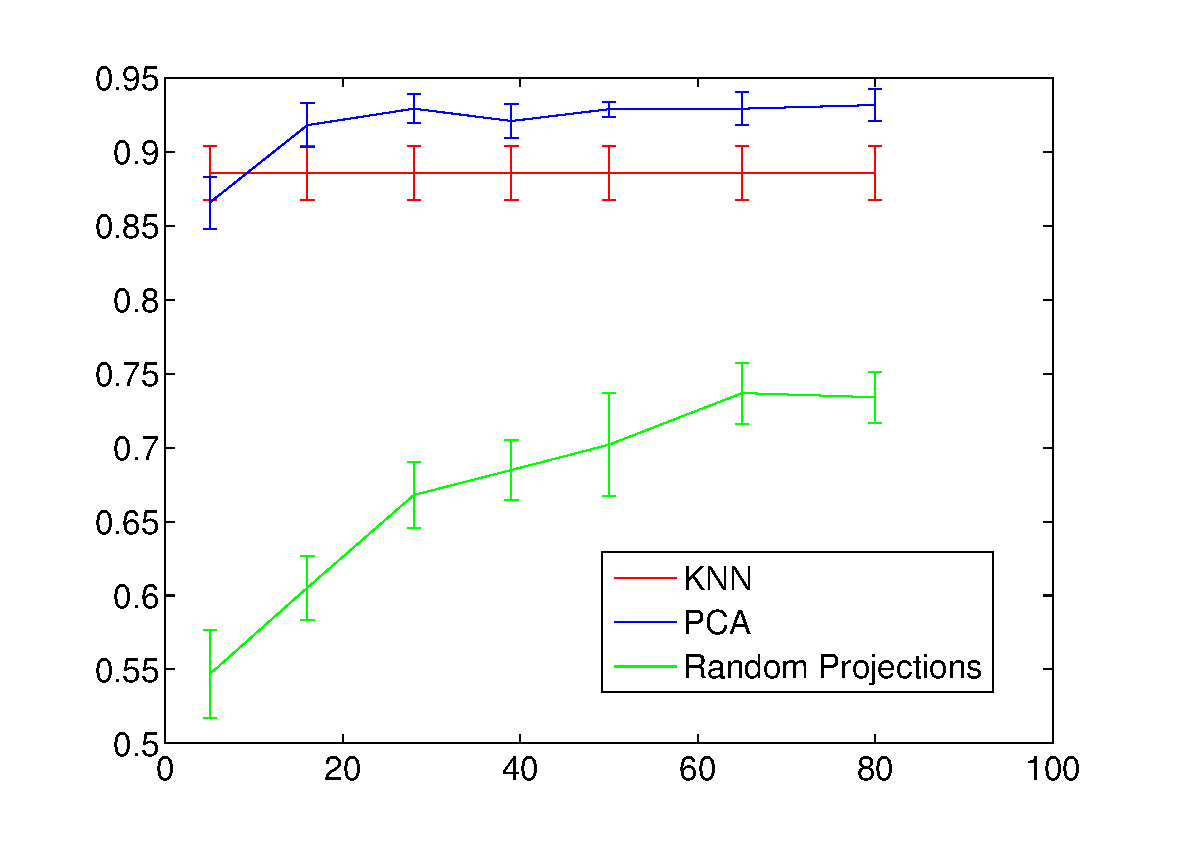
\includegraphics[width=.5\textwidth]{../images/knnVpcaVrproj.eps}}
\subfloat[Accuracy vs Dim. proj  with linear and RBF SVM]{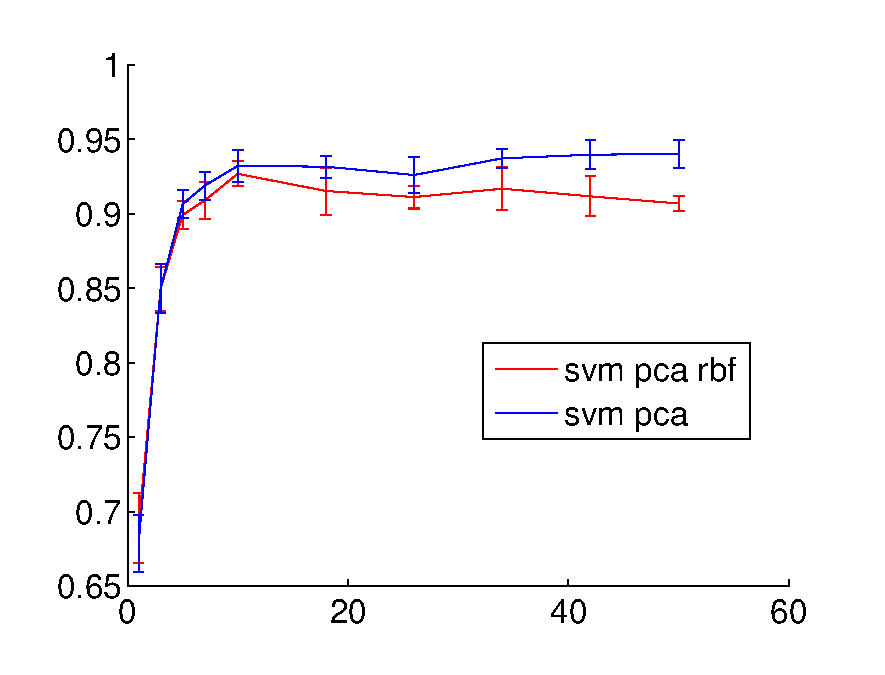
\includegraphics[width=.5\textwidth]{../images/svm_linear_vs_rbf.eps}}
\caption{Curse of Dimensionality and Distance-Based Classification}
\label{fig:distance}
\end{figure}

%\end{document}
